\section{Ziel}
\label{sec:Ziel}
Mit diesem Experiment soll der Prozess der Phasenumwandlung von Wasser untersucht werden. Dazu wird die Dampfdruckkurve gemessen und die Verdampfungswärme $L$ bestimmt. Die Verdampfungswärme wird
dabei auf ihre Temperaturabhängigkeit untersucht.
\section{Theorie}
\label{sec:Theorie}
Damit dieses Ziel erreicht werden kann, muss zunächst verstanden werden was die Dampfdruckkurve beschreibt. Dies wird nun durch ein Beispiel mit Wasser erleutert.
Wasser nimmt mit variirender Temperatur unterschiedliche Aggregatzustände an. Ein Aggregatzustand beschreibt soetwas wie die Bewegungen der Teilchen eines Stoffen in einem bestimmten Volumen.
Die auf der Erde typischen Aggregatzustände sind fest, flüssig und gasförmig. Allerdings ist der Aggregatzustand eines Stoffes nicht nur temperaturabhängig. Der Umgebungsdruck eines Stoffes 
beeinflusst ebenfalls den Aggregatzustand. Durch diese beiden Abhängigkeiten lässt sich für einen Stoff ein Druck-Temperatur-Diagramm zeichnen. Ein solches Diagramm ist in \autoref{fig:phasenabbildung}
dargestellt.
\begin{figure}
    \centering
    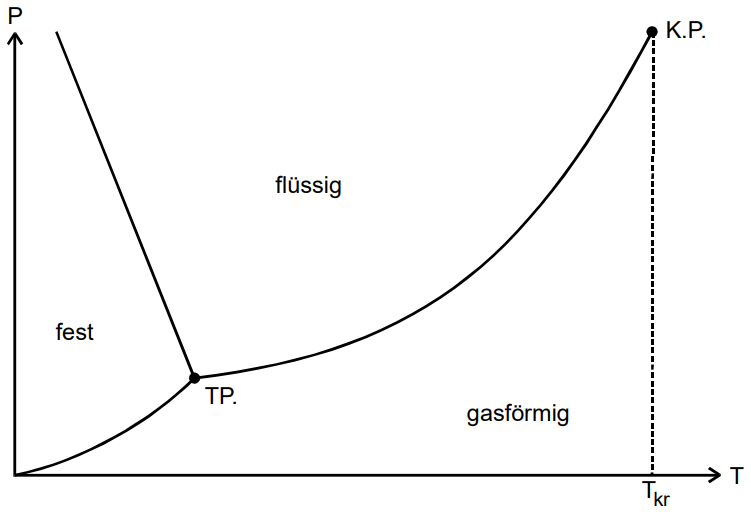
\includegraphics[width=\textwidth]{content/Phasenabbildung.PNG}
	\caption{In dieser Abbildung ist ein quantitatives Zustandsdiagramm von Wasser dargestellt. \cite{v203}}
	\label{fig:phasenabbildung}
\end{figure}
Untersucht man nun den Aggregatzustand von Wasser zu verschiedenen Temperaturen und Drücken ergeben sich drei Bereiche im Diagramm, jeweils einer pro Aggregatzustand.  Diese sind durch Grenzen
getrennt, wie man in \autoref{fig:phasenabbildung} erkennen kann. Die Kurve zwischen den Bereichen der Aggregatzustände flüssig und gasförmig wird Dampfdruckkurve genannt. An genau dieser Grenze besitzt das System
nur noch einen Freiheitsgrad, da bei Vorgabe eines Parameters der andere eindeutig definiert ist. Eine wichtige Charakteristik der Dampfdruckkurve ist, dass sie im wesentlichen durch die 
Verdampfungswärme $L$ beschrieben werden kann. Die Verdampfungswärme ist eine wichtige Eigenschaft von Stoffen. In gewissen Temperauturbereichen kann sie zwar als Konstante genähert werden,
allerdings ist sie im allgemeinen eine temperaturabhängige Größe. 
\subsection{mikroskopische Vorgänge bei der Verdampfung und Kondensation}
\label{subsec:T_VK}
In diesem Verusch wird mit einer Flüssigkeit in einem evakuiertem Gefäß gearbeitet. Eine Flüssigkeit in einem evakuierten Gefäß verdampft solange bis der Druck in dem Gefäß einen Wert erreicht,
der im Zustandsdiagramm im "flüssigen" Bereich liegt. Daher werden im Folgendem die mikroskopischen Vorgänge bei Verdampfung und Kondensation erklärt. Bei dem eben genannten Verdampfungsprozess
geht ein Stoff vom flüssigen Zustand in den gasförmigen über. Dabei "verlassen" diejenigen Moleküle die Flüssigkeit, welche gemäß der Maxwellschen Geschwindigkeitsverteilung die maximale kinetische 
Energie besitzen. Bei diesem Vorgang kann sich vorgestellt werden, dass die Moleküle aufgrund ihrer Geschwindigkeit einfach aus der Flüssigkeitsoberfläche herausschießen. Damit das geschieht muss
ein Molekül aber zunächst die molekulare Bindungsenergie überwinden. Daher muss ein Molekül um zu verdampfen entweder eine externe energetische Anregung bekommen oder die notwendige Energie
dem Wärmereservior der Flüssigkeit entnehmen. Aufgrund dieser mikroskopischen Überlegung definiert man eine Größe $L_{mol}$ der Einheit Joule/Mol, welche man molare Verdampfungswärme nennt. Diese beschreibt die nötige Energie
um ein Mol einer Flüssigkeit in Dampf gleicher Temperatur umzuwandeln. Sollte ein solches Mol an Gas wieder Kondensieren, also vom gasförmigen Zustand wieder in den flüssigen wechseln, wird genau
die Energie $L_{mol}$ wieder frei beziehungsweise geht dann in das Wärmereservoir der Flüssigkeit über. Da der Druck vom Gas durch Stöße mit der Umgebung gebildet wird kann es auch passieren, dass
die Gasmoleküle mit der Flüssigkeitsoberfläche zusammenstoßen und dann wieder in die Flüssigkeit aufgenommen werden, also Kondensieren. Diese Vorgänge von Verdampfung und Kondensation finden immer statt.
Aber nach hinreichendlanger Zeit bildet sich zwischen diesen Prozessen ein Gleichgewicht. Da der Verdampfungsprozess nicht mehr beobachtet werden kann spricht man bei diesem Gleichgewicht
davon, dass "Flüssigkeit und Dampf koexistieren". Daher bildet sich im Gas ein konstanter Druck. Dieser wird Sättigungsdampfdruck genannt. Er muss mit zunehmender Temperatur ansteigen, da bei
erhöhter kinetischer Energie die Moleküle häufiger Stoßen und da mehr Moleküle aus der Flüssigkeit austreten können. Der Sättigungsdampfdruck hängt nicht vom Volumen des Gefäßes ab. Daher kann 
das gesättigte Gas nicht durch die Allgemeine Gasgleichung beschrieben werden.
\subsection{Differentielgleichung einer Dampfdruckkurve}
\label{subsec:T_DGL}
Damit die Dampfdruckkurve nicht nur durch expermientelle Regressionen dargestellt werden kann ist es von Interesse eine theoretische Beschreibung der Dampfdruckkurve zu finden. Dazu wird 
ein reversibler Kreisprozess von Verdampfung und Kondensation betrachtet. Dieser wird in \autoref{fig:kreisprozess} dargestellt.
\begin{figure}
    \centering
    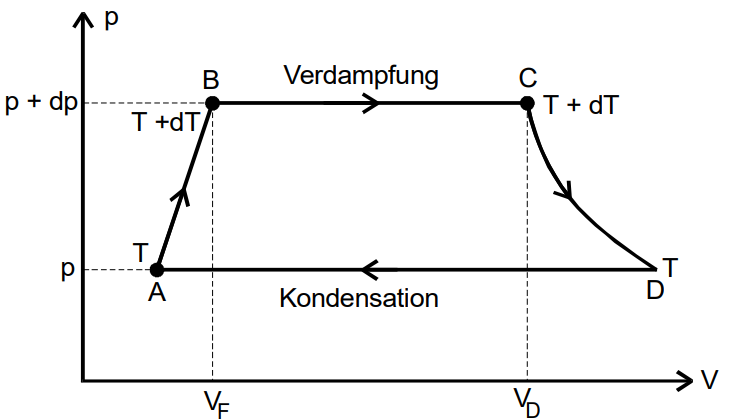
\includegraphics[width=\textwidth]{content/kreisprozess.PNG}
	\caption{In dieser Abbildung ist ein Verdampfungs-Kondensations-Kreisprozess dargestellt. \cite{v203}}
	\label{fig:kreisprozess}
\end{figure}
Wie im \autoref{subsec:T_VK} beschrieben wird bei Kondensation und Verdampfung Energie benötigt sowie auch Energie abgegeben. Durch Aufstellen von Formeln für Arbeiten und Wärmemengen kann mit Hilfe
der Hauptsätze der Thermodynamik die Differentielgleichung 
\begin{equation}
    \label{eqn:DGL1}
    \left(V_\text{D} - V_\text{F}\right)\symup{d}p = \frac{L}{T}\symup{d}T
\end{equation}
aufgestellt werden dessen Lösung die Dampfdruckkurve eines Stoffes beschreibt. $V_\text{D}$ beschreibt dabei das Volumen des Gases und $V_\text{F}$ das der Flüssigkeit.
Diese Differentielgleichung wird Clausius-Clapeyronsche Gleichung genannt.
\subsection{Integration der Clausius-Clapeyronschen Gleichung durch vereinfachende Annahmen}
\label{subsec:T_int}
Die Integration der Clausius-Clapeyronschen Gleichung ist im allgemeinen Fall schwierig, da sie durch kompliziert Temperaturabhängigkeiten ausgedrückt wird. Daher werden Näherungen benötigt, welche
die Integration vereinfache oder ermöglichen. Daher soll in guter Näherung gelten, dass $V_\text{F}$ gegenüber $V_\text{D}$ vernachlässigbar klein ist. Außerdem muss $V_\text{D}$ die ideale Gasgleichung
\begin{equation}
    \label{eqn:V_D}
    V_\text{D}(p,T) = R\frac{T}{p}
\end{equation} 
erfüllen. Die Verdampfungswärme $L$ darf dafür nicht druck- und temperaturabhängig sein. Diese Näherungen können aber nur als hinreichend genau betrachtet werden solange die Temperatur
viel kleiner ist als die kritische Temperatur. Also gilt $T \ll T_\text{kr}$. Diese kritische Temperatur $T_\text{kr}$ ist in \autoref{fig:phasenabbildung} eingezeichnet. Er beschreibt die "obere"
Temperaturgrenze der Dampfdruckkurve. Druch die Annahmen kann nun die Differentielgleichung integriert werden. Daher ergibt sich aus \autoref{eqn:DGL1} und Annahme der \autoref{eqn:V_D} durch Integration
\autoref{eqn:int}.
\begin{equation}
    \label{eqn:int}
    p = p_0\text{e}^{-\frac{L}{RT}}
\end{equation}
Da \autoref{eqn:int} nur noch von den Variablen $p$ und $T$ abhängt lässt sich diese Gleichung nach Variablen trennen. Daraus folgt dann 
\begin{equation}
    \label{eqn:gerade}
    \text{ln}\left(\frac{p}{p_0}\right) = -\frac{L}{R}\frac{1}{T}.
\end{equation}
Diese Gleichung besitzt die Form einer Geradengleichung der Variablen $\text{ln}\left(\frac{p}{p_0}\right)$ und $\frac{1}{T}$ mit der Steigung $-\frac{L}{R}$. Daher kann aus \autoref{eqn:gerade} die 
Verdampfungswärme $L$ bestimmt werden. Aus dieser kann wiederum die innere Verdampfungswärme $L_\text{i}$ bestimmen.
\begin{equation}
    \label{eqn:LI}
    L_\text{i} = L - L_\text{a}
\end{equation}
Dabei beschreibt $L_\text{a}$ die äußere Verdampfungswärme.